\newpage

\subsubsection{UCS 9 - Gestione degli amministratori}%sea level

\begin{figure}[h!]
    \centering
      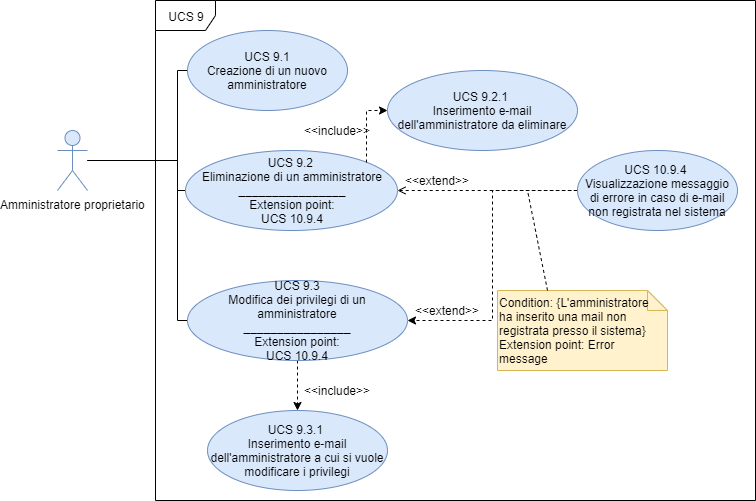
\includegraphics[scale=0.5]{Sezioni/UseCase/Immagini/UCS9.png}
    \caption{UCS 9 - Gestione degli amministratori}
  \end{figure}
\begin{itemize}

\item \textbf{Attori primari:} Amministratore proprietario
%\item \textbf{Attori secondari:}%opzionale
\item \textbf{Precondizione:} L'amministratore è autenticato presso il sistema.
\item \textbf{Postcondizione:} L'amministratore ha eseguito l'azione desiderata tra: nomina di un amministratore, eliminazione di un amministratore e modifica dei privilegi di un amministratore.
\item \textbf{Scenario principale:} L'amministratore ha la possibilità di gestire i propri amministratori.
\item \textbf{Scenario alternativo:} L'amministratore seleziona la funzionalità per annullare le modifiche agli amministratori [UCS 9.4].
\item \textbf{Flusso di eventi:} %elenco puntato
  \begin{enumerate}
        \item L'amministratore seleziona la funzionalità per la gestione degli amministratori;
        \item L'amministratore seleziona una funzionalità tra: nomina di un amministratore [UCS 9.1] [UCS 9.5], eliminazione di un amministratore [UCS 9.2] e modifica dei privilegi di un amministratore [UCS 9.3].
    \end{enumerate}
\item \textbf{Estensioni:}
	\begin{itemize}
		\item UCS 9.4 - Annullamento modifiche agli amministratori.
	\end{itemize}
\end{itemize}


\subsubsection{UCS 9.1 - Nomina di un nuovo amministratore}%sea level

\begin{figure}[h!]
  \centering
    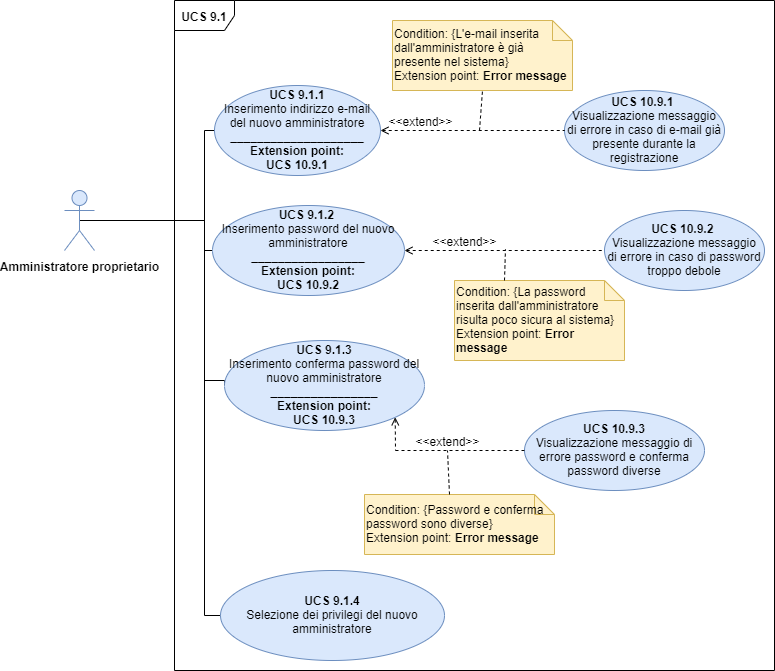
\includegraphics[scale=0.5]{Sezioni/UseCase/Immagini/UCS9.1.png}
  \caption{UCS 9.1 - Nomina di un nuovo amministratore}
\end{figure}

\begin{itemize}
\item \textbf{Attori primari:} Amministratore proprietario
%\item \textbf{Attori secondari:}%opzionale
\item \textbf{Precondizione:} L'amministratore è autenticato presso il sistema e si trova nella funzionalità di gestione degli amministratori.
\item \textbf{Postcondizione:} L'amministratore ha creato un account per il nuovo amministratore, il quale è stato registrato presso il sistema.
\item \textbf{Scenario principale:} L'amministratore compila il modulo per la nomina del nuovo amministratore.
\item \textbf{Flusso di eventi:} %elenco puntato
  \begin{enumerate}
        \item Inserimento indirizzo e-mail [UCS 9.1.1];
        \item Inserimento password [UCS 9.1.2];
        \item Inserimento conferma password [UCS 9.1.3];
        \item Selezione dei privilegi del nuovo amministratore [UCS 9.1.4]. Si dovrà scegliere tra "Visualizzatore" e "Gestore".
    \end{enumerate}
\item \textbf{Estensioni:}
	\begin{itemize}
		\item UCS 10.9.1 - Visualizzazione messaggio di errore in caso di e-mail già presente durante la registrazione;
		\item UCS 10.9.2 - Visualizzazione messaggio di errore in caso di password troppo debole;
		\item UCS 10.9.3 - Visualizzazione messaggio di errore in caso di password e conferma password diverse.
	\end{itemize}
\end{itemize}

\subsubsection{UCS 9.1.1 - Inserimento e-mail}
\begin{itemize}
\item \textbf{Attori primari:} Amministratore proprietario
\item \textbf{Precondizione:} L'amministratore si trova nella funzionalità per la nomina di un nuovo amministratore.
\item \textbf{Postcondizione:} L'utente ha inserito l'e-mail per l'account del nuovo amministratore.
\item \textbf{Scenario principale:} Inserimento dell'email per il nuovo amministratore.
\end{itemize}

\subsubsection{UCS 9.1.2 - Nuova password}
\begin{itemize}
\item \textbf{Attori primari:} Amministratore proprietario
\item \textbf{Precondizione:}  L'amministratore si trova nella funzionalità per la nomina di un nuovo amministratore.
\item \textbf{Postcondizione:} L'amministratore ha inserito la nuova password per il nuovo amministratore.
\item \textbf{Scenario principale:} Inserimento della password per il nuovo amministratore.
\end{itemize}

\subsubsection{UCS 9.1.3 - Conferma nuova password}
\begin{itemize}
\item \textbf{Attori primari:} Amministratore proprietario
\item \textbf{Precondizione:} L'amministratore si trova nella funzionalità per la nomina di un nuovo amministratore.
\item \textbf{Postcondizione:} L'amministratore ha reinserito la nuova password nel campo di conferma password.
\item \textbf{Scenario principale:} Inserimento della conferma della password per il nuovo amministratore.
\end{itemize}

\subsubsection{UCS 9.1.4 - Selezione dei privilegi del nuovo amministratore}
\begin{itemize}
\item \textbf{Attori primari:} Amministratore proprietario
\item \textbf{Precondizione:} L'amministratore si trova nella funzionalità per la nomina di un nuovo amministratore.
\item \textbf{Postcondizione:} L'amministratore ha selezionato tra "Visualizzatore" e "Gestore" come privilegi garantiti al nuovo amministratore da nominare.
\item \textbf{Scenario principale:} Selezione dei privilegi per il nuovo amministratore.
\end{itemize}

\subsubsection{UCS 9.2 - Eliminazione di un amministratore}%sea level

\begin{figure}[h]
  \centering
    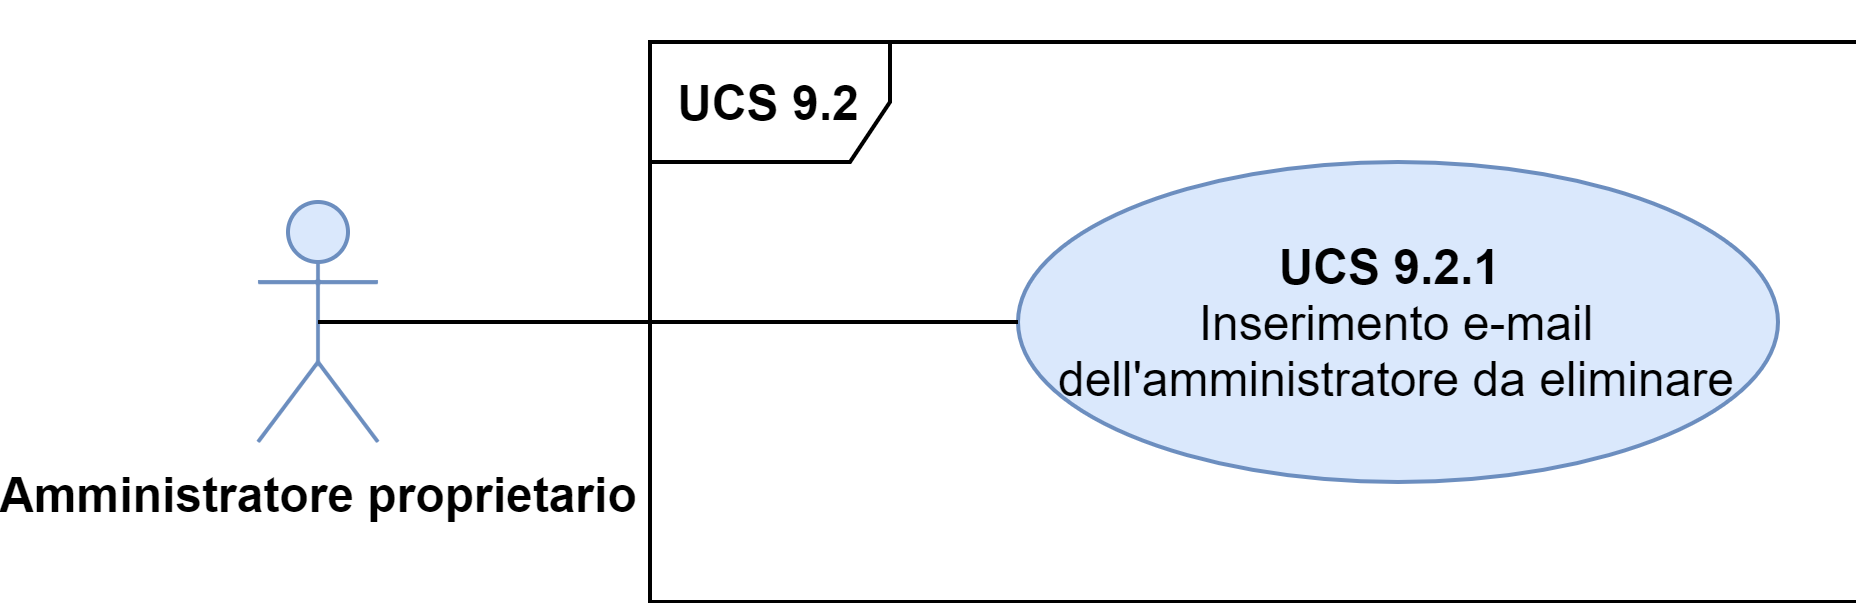
\includegraphics[scale=1.0]{Sezioni/UseCase/Immagini/UCS9.2.png}
  \caption{UCS 9.2 - Eliminazione di un amministratore}
\end{figure}

\begin{itemize}
\item \textbf{Attori primari:} Amministratore proprietario
%\item \textbf{Attori secondari:}%opzionale
\item \textbf{Precondizione:} L'amministratore è autenticato presso il sistema e si trova nella funzionalità di gestione degli amministratori.
\item \textbf{Postcondizione:} L'amministratore ha rimosso i permessi dell'amministratore identificato dall'e-mail inserita.
\item \textbf{Scenario principale:} L'amministratore inserisce l' email dell'amministratore al quale vuole togliere i permessi e quindi conferma la scelta.
\item \textbf{Scenario alternativo:} L'amministratore inserisce un e-mail che non è registrata presso il sistema, verrà pertanto mostrato un messaggio d'errore [UCS 10.9.4].
\item \textbf{Flusso di eventi:} %elenco puntato
  \begin{enumerate}
        \item Inserimento e-mail del profilo dell'amministratore da rimuovere [UCS 9.2.1];
        \item L'amministratore gli rimuove i permessi di amministrazione dell'organizzazione;
        \item L'amministratore seleziona la funzionalità di conferma.
    \end{enumerate}
\item \textbf{Estensioni:}
	\begin{itemize}
		\item UCS 10.9.4 - Visualizzazione messaggio di errore in caso di e-mail non registrata nel sistema.
	\end{itemize}
\end{itemize}

\subsubsection{UCS 9.2.1 - Inserimento e-mail dell'amministratore da eliminare}%fish level
\begin{itemize}
\item \textbf{Attori primari:} Amministratore proprietario
%\item \textbf{Attori secondari:}%opzionale
\item \textbf{Precondizione:} L'amministratore è nella funzionalità "Eliminazione di un amministratore".
\item \textbf{Postcondizione:} L'amministratore ha inserito una l'e-mail dell'amministratore da eliminare.
\item \textbf{Scenario principale:} Inserimento e-mail dell'amministratore da eliminare.
\end{itemize}

\subsubsection{UCS 9.3 - Modifica dei privilegi di un amministratore}%sea level

\begin{figure}[h]
  \centering
    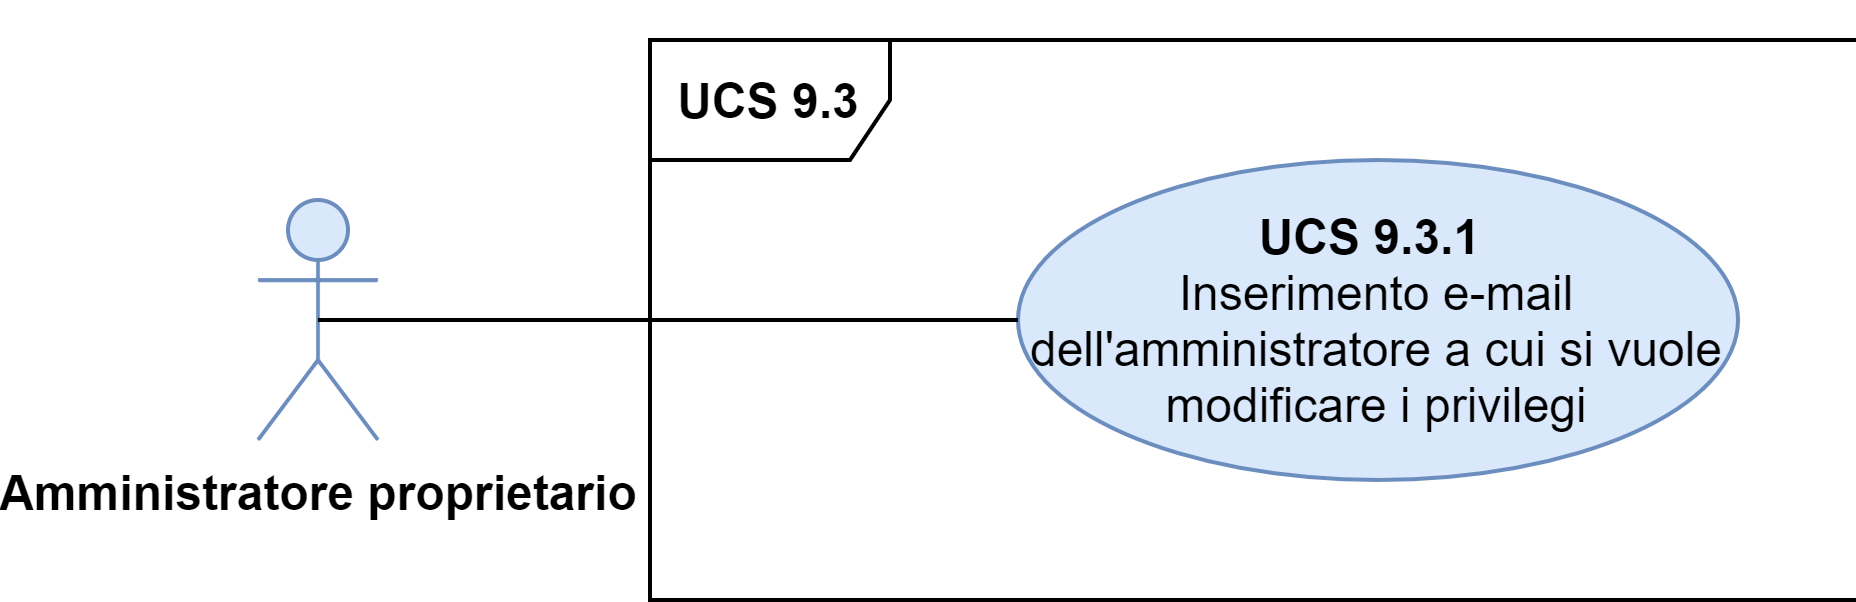
\includegraphics[scale=1.0]{Sezioni/UseCase/Immagini/UCS9.3.png}
  \caption{UCS 9.3 - Modifica dei privilegi di un amministratore}
\end{figure}

\begin{itemize}
\item \textbf{Attori primari:} Amministratore proprietario
%\item \textbf{Attori secondari:}%opzionale
\item \textbf{Precondizione:} L'amministratore è autenticato presso il sistema e si trova nella funzionalità di gestione degli amministratori.
\item \textbf{Postcondizione:} L'amministratore ha modificato i privilegi dell'amministratore identificato dalla password inserita.
\item \textbf{Scenario principale:} L'amministratore inserisce la mail dell'amministratore a cui vuole modificarne i privilegi e quindi sceglie il privilegio da assegnargli.
\item \textbf{Flusso di eventi:} %elenco puntato
  \begin{enumerate}
        \item Inserimento e-mail del profilo dell'amministratore da rimuovere [UCS 9.3.1];
        \item L'amministratore seleziona i nuovi privilegi da assegnare all'amministratore, potrà scegliere se assegnare "Gestore" oppure "Visualizzatore".
    \end{enumerate}
\item \textbf{Estensioni:}
	\begin{itemize}
		\item UCS 10.9.4 - Visualizzazione messaggio di errore in caso di e-mail non registrata nel sistema.
	\end{itemize}
\end{itemize}

\subsubsection{UCS 9.3.1 - Inserimento e-mail dell'amministratore a cui si vuole modificare i privilegi}%fish level
\begin{itemize}
\item \textbf{Attori primari:} Amministratore proprietario
%\item \textbf{Attori secondari:}%opzionale
\item \textbf{Precondizione:} L'amministratore è nella funzionalità "Modifica dei privilegi di un amministratore".
\item \textbf{Postcondizione:} L'amministratore ha inserito una l'e-mail dell'amministratore a cui vuole modificare i privilegi.
\item \textbf{Scenario principale:} Inserimento e-mail dell'amministratore a cui si vuole modificare i privilegi.
\end{itemize}

\subsubsection{UCS 9.4 - Annullamento modifiche agli amministratori}%sea level

\begin{itemize}
\item \textbf{Attori primari:} Amministratore proprietario
%\item \textbf{Attori secondari:}%opzionale
\item \textbf{Precondizione:} L'amministratore è autenticato presso il sistema e si trova nella funzionalità di gestione degli amministratori.
\item \textbf{Postcondizione:} L'amministratore annullato le modifiche che stava apportando agli amministratori.
\item \textbf{Scenario principale:} L'amministratore seleziona la funzionalità di annullamento modifiche.
\end{itemize}

\subsubsection{UCS 9.5 - Nomina di un nuovo amministratore già presente nel sistema}%sea level

\begin{figure}[h!]
    \centering
      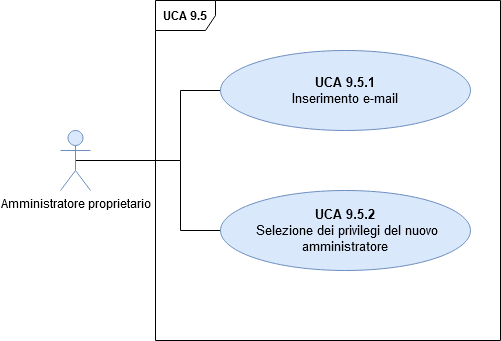
\includegraphics[scale=0.5]{Sezioni/UseCase/Immagini/UCS9.5.png}
    \caption{UCS 9.5 - Nomina di un nuovo amministratore già presente nel sistema}
  \end{figure}


\begin{itemize}
\item \textbf{Attori primari:} Amministratore proprietario
%\item \textbf{Attori secondari:}%opzionale
\item \textbf{Precondizione:} L'amministratore è autenticato presso il sistema e si trova nella funzionalità di gestione degli amministratori.
\item \textbf{Postcondizione:} L'amministratore ha nominato un account già presente nel sistema come amministratore della propria organizzazione.
\item \textbf{Scenario principale:} L'amministratore compila il modulo per nominare un account già presente nel sistema come amministratore della propria organizzazione.
\item \textbf{Flusso di eventi:} %elenco puntato
  \begin{enumerate}
        \item Inserimento indirizzo e-mail [UCS 9.5.1];
        \item Selezione dei privilegi del nuovo amministratore [UCS 9.5.2]. Si dovrà scegliere tra "Visualizzatore" e "Gestore".
    \end{enumerate}
\end{itemize}

\subsubsection{UCS 9.5.1 - Inserimento e-mail}
\begin{itemize}
\item \textbf{Attori primari:} Amministratore proprietario
\item \textbf{Precondizione:} L'amministratore si trova nella funzionalità per la nomina di un nuovo amministratore già presente nel sistema.
\item \textbf{Postcondizione:} L'utente ha inserito l'e-mail per l'account del nuovo amministratore.
\item \textbf{Scenario principale:} Inserimento dell'email per il nuovo amministratore.
\end{itemize}


\subsubsection{UCS 9.5.2 - Selezione dei privilegi del nuovo amministratore}
\begin{itemize}
\item \textbf{Attori primari:} Amministratore proprietario
\item \textbf{Precondizione:} L'amministratore si trova nella funzionalità per la nomina di un nuovo amministratore già presente nel sistema.
\item \textbf{Postcondizione:} L'amministratore ha selezionato tra "Visualizzatore" e "Gestore" come privilegi garantiti al nuovo amministratore da nominare.
\item \textbf{Scenario principale:} Selezione dei privilegi per il nuovo amministratore.
\end{itemize}
